\section{Results}\label{sec:results}

To draw meaningful conclusions we created several types of visualization of the data. First and foremost we plotted the open events onto a map - either as a point map or as a occurrences distribution map for each city district. 

\begin{figure}[!htp]
	\includegraphics[width=1\linewidth]{images/Barcelona_points.png}
	\caption{Snippet of Barcelona with Open Events}\label{fig:barcelonapoints}	
\end{figure}

\begin{figure}[!htp]
	\includegraphics[width=1\linewidth]{images/Barcelona_points_Language.png}
	\caption{Snippet of Barcelona with Language \& Ethnic Identity Events}\label{fig:barcelonapointslanguage}	
\end{figure}

In Figure \ref{fig:barcelonapoints} one can see an example of Barcelona with open events plotted as points. The different colors represent different meetup categories. 

\begin{figure}[!htp]
	% Maximum length
	\subfloat[Activity per District]{\label{fig1:a}\includegraphics[width=0.49\linewidth]{images/activities_of_districts/Barcelona.png}}\hfill
	\subfloat[Activity per Capita per District]{\label{fig1:b}\includegraphics[width=0.49\linewidth]{images/activities_per_capita_of_districts/Barcelona.png}}%
	\caption{Barcelona}\label{fig:barcelonamap}
\end{figure}

\begin{figure}[!htp]
	% Maximum length
	\subfloat[Activity per District]{\label{fig1:a}\includegraphics[width=0.49\linewidth]{images/activities_of_districts/London.png}}\hfill
	\subfloat[Activity per Capita per District]{\label{fig1:b}\includegraphics[width=0.49\linewidth]{images/activities_per_capita_of_districts/London.png}}%
	\caption{London}
\end{figure}

\begin{figure}[!htp]
	% Maximum length
	\subfloat[Activity per District]{\label{fig1:a}\includegraphics[width=0.49\linewidth]{images/activities_of_districts/Berlin.png}}\hfill
	\subfloat[Activity per Capita per District]{\label{fig1:b}\includegraphics[width=0.49\linewidth]{images/activities_per_capita_of_districts/Berlin.png}}%
	\caption{Berlin}
\end{figure}

\begin{figure}[!htp]
	% Maximum length
	\subfloat[Activity per District]{\label{fig1:a}\includegraphics[width=0.49\linewidth]{images/activities_of_districts/Madrid.png}}\hfill
	\subfloat[Activity per Capita per District]{\label{fig1:b}\includegraphics[width=0.49\linewidth]{images/activities_per_capita_of_districts/Madrid.png}}%
	\caption{Madrid}
\end{figure}

\begin{figure}[!htp]
	% Maximum length
	\subfloat[Activity per District]{\label{fig1:a}\includegraphics[width=0.49\linewidth]{images/activities_of_districts/Paris.png}}\hfill
	\subfloat[Activity per Capita per District]{\label{fig1:b}\includegraphics[width=0.49\linewidth]{images/activities_per_capita_of_districts/Paris.png}}%
	\caption{Paris}
\end{figure}

\begin{figure}[!htp]
	% Maximum length
	\subfloat[Activity per District]{\label{fig1:a}\includegraphics[width=0.49\linewidth]{images/activities_of_districts/Brussels.png}}\hfill
	\subfloat[Activity per Capita per District]{\label{fig1:b}\includegraphics[width=0.49\linewidth]{images/activities_per_capita_of_districts/Brussels.png}}%
	\caption{Brussels}
\end{figure}

\begin{figure}[!htp]
	% Maximum length
	\subfloat[Activity per District]{\label{fig1:a}\includegraphics[width=0.49\linewidth]{images/activities_of_districts/Hamburg.png}}\hfill
	\subfloat[Activity per Capita per District]{\label{fig1:b}\includegraphics[width=0.49\linewidth]{images/activities_per_capita_of_districts/Hamburg.png}}%
	\caption{Hamburg}
\end{figure}

\begin{figure}[!htp]
	% Maximum length
	\subfloat[Activity per District]{\label{fig1:a}\includegraphics[width=0.49\linewidth]{images/activities_of_districts/NewYork.png}}\hfill
	\subfloat[Activity per Capita per District]{\label{fig1:b}\includegraphics[width=0.49\linewidth]{images/activities_per_capita_of_districts/NewYork.png}}%
	\caption{New York City}
\end{figure}

\begin{figure}[!htp]
	% Maximum length
	\subfloat[Activity per District]{\label{fig1:a}\includegraphics[width=0.49\linewidth]{images/activities_of_districts/Munich.png}}\hfill
	\subfloat[Activity per Capita per District]{\label{fig1:b}\includegraphics[width=0.49\linewidth]{images/activities_per_capita_of_districts/Munich.png}}%
	\caption{Munich}
\end{figure}

\begin{figure}[!htp]
	% Maximum length
	\subfloat[Activity per District]{\label{fig1:a}\includegraphics[width=0.49\linewidth]{images/activities_of_districts/HongKong.png}}\hfill
	\subfloat[Activity per Capita per District]{\label{fig1:b}\includegraphics[width=0.49\linewidth]{images/activities_per_capita_of_districts/HongKong.png}}%
	\caption{Hong Kong}\label{fig:hongkongmap}
\end{figure}